\section{Microcontroller}

Til projektet skal bruges en microcontroller som skal håndtere følgende opgaver:  
\begin{itemize}
	\item Linklag mellem 3G modul og fight control board
	\item Processering af billeder og evt. komprimering.
	\item Læsning fra de forskellige sensorer.
	\item Beregne dronens næste handling. 
	\begin{itemize}
		\item Ud fra nuværende position og ønsket position.
		\item Sørge for at ændre orientering på drone. 
	\end{itemize}
\end{itemize}

\vspace{0.5cm}

Microcontrolleren skal kunne håndtere C++ kode, da det ønskes at programmere objekt orienteret. C++ giver et højt abstraktions niveau og gør det muligt at bruge klasser og objekter. Hvilket generelt giver en bedre kodestruktur og gør koden nærmere at overskue.

Desuden skal mircocontrolleren være kompatibel med det 3G-shield der er beskrevet i afsnittet \textit{3G/GPS shield}. 

Både Raspberry Pi og Arduino kan håndtere C++ og er kompatible med 3G-shieldet. Raspberry Pi og Arduino microcontrollere ens på mange punkter. Dog har Raspberry Pi en noget kraftigere processor og besidder nogle unødvendige funktioner. 

Det blev besluttet at bruge et Arduino 2560 board\footnote{http://arduino.cc/en/Main/arduinoBoardMega2560}. Hovedsageligt blev denne microcontroller valgt, da Raspberry Pi krævede en form for mellemlags board og fordi det var muligt at låne Arduino 2560 af Ingeniørhøjskolen. 

\vspace{0.5cm}

\begin{figure}[H]
\centering
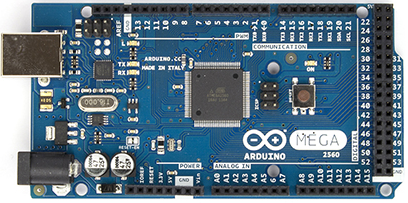
\includegraphics[width=0.5\textwidth]{Billeder/ArduinoMega2560.png}
\caption{Arduino 2560}
\label{fig:Arduino_2560}
\end{figure}


